\section{\cnet{} v3: contaminant-aware lens finding and Euclid cross-validation}
\label{sec:v3}
The v2 DR9 sweep ended in a decisive negative (\S\ref{sec:campaign}): of 601 genuinely-new
group-conformal candidates, \emph{zero} were graded A/B by either independent vetter, and the only
five graded $\ge$B were already-catalogued lenses. The candidates were overwhelmingly luminous-red
galaxies with companions, rings, and blends. This diagnoses the binding constraint precisely: it is
not architecture (the v1/v2 finding) but \emph{lens-vs-mimic separation} and \emph{vetting
resolution}. The field-wide remedy is the same --- contaminant-targeted hard negatives give an
$11\times$ false-positive reduction at $2.3\%$ true-positive cost \citep{staf327}. v3 builds a
contaminant-aware finder, deploys it on DR10/DR11, and cross-validates the overlap against Euclid
Q1. We keep all v1/v2 numbers; v3 is additive, and every number below is read from a tracked
artifact under \texttt{data/v3/} or \texttt{v3/}.

\paragraph{The mimic metric and the v2 baseline (A0).} The v1/v2 headline measured recovery at a
false-positive rate set against \emph{random} galaxies; the campaign showed that is the wrong null.
We define \textbf{recovery@matched-mimic-FPR}: identical arithmetic, but the negative class is a
bank of lens-\emph{mimics} rather than random galaxies. Against this null the shipped v2-lean
ensemble --- which recovers $96$--$100\%$ of held-out lenses at random-FPR --- recovers only
$0.168$ (Storfer) / $0.307$ (Inchausti) at mimic-FPR $0.05$ on the curated 601-mimic seed bank.
The mimic-discrimination gap, not random-galaxy recovery or architecture, is what v3 must close.

\paragraph{The lens-mimic bank (A1).} Rather than mine a fresh pool we reuse the DR10 sweep:
$148{,}034$ NEW survivors are CNN-high, DR10-native non-lenses, morphology-typed by joining the
Tractor catalogue (extended-LRG $34$\,k --- the \citet{staf327} regime --- plus
compact-REX, exp-disk, and the campaign's fine types). A 120-row stratified agentic G1 gate
confirms $98.3\%$ non-lens purity. The bank is $118{,}901$ training rows $+$ a frozen,
stratified $29{,}724$-row held-out mimic-eval that never enters training.

\paragraph{Contaminant-aware retraining (A2).} We retrain the three swappable members with the
v2 ``hard'' recipe held \emph{byte-identical} (same $n_{\rm mine}{=}10{,}000$ displaced bootstrap
negatives, same per-member seed) and change only the negative \emph{content}: a fraction $f$ of the
displaced negatives become typed mimics from the bank. A blend-fraction sweep selects $f{=}0.5$
($f{=}0.7$ over-specialises). On the held-out DR10 mimic-eval (Table~\ref{tab:a2}) v3blend8 lifts
Storfer mimic-recovery from $0.713\!\to\!0.790$ at $0.05$ and $0.460\!\to\!0.699$ at $0.01$, with
the largest per-type gains on the dominant lrg\_companion/extended-LRG contaminants. The cost is a
small, real drop in \emph{random}-galaxy recall ($0.967\!\to\!0.935$ Storfer at random-FPR$\,0.01$)
--- exactly the \citet{staf327} trade.

\paragraph{Ensemble refit and the lens-vs-mimic head (A6, A3).} A roster search over the average
combiner finds \textbf{v3blend8} --- keeping \emph{both} the v2-hard and v3-mimic-blended version
of each member --- is near-Pareto: it recovers random-FPR recall to within CI of v2-lean while
roughly doubling mimic-recovery. (The $194$\,K-free l18 ResNet is, by contrast, dead weight for
mimic separation; dropping it maximises mimic-recovery at a $3\%$ random-recall cost.) A learned
logistic \emph{lens-vs-mimic head} on the eight member scores tops every average roster at the
$\phi{=}0.05$ operating point, but it overfits the strict tail and --- as \S\ref{sec:v3limits}
shows --- does not generalise to the independent Euclid test, so the deployable model is
\textbf{v3blend8}, with the head as a $\phi{=}0.05$ stage-2 re-ranker.

\begin{table}[t]\centering
\caption{A2 contaminant-aware retraining (mimic-blend $f{=}0.5$), v2-lean$\to$v3blend8, on the held-out DR10 mimic-eval. Mimic-recovery rises at every operating point; the random-galaxy recall (testneg null) drops only slightly (the staf327 trade).}
\label{tab:a2}\small
\begin{tabular}{lcccc}
\toprule
 & \multicolumn{2}{c}{recovery@mimic-FPR (Storfer)} & \multicolumn{2}{c}{recovery@random-FPR(0.01)}\\
\cmidrule(lr){2-3}\cmidrule(lr){4-5}
 & @0.05 & @0.01 & Storfer & Inchausti\\
\midrule
v2-lean & 0.713 & 0.460 & 0.967 & 0.998\\
v3blend8 & \textbf{0.793} & \textbf{0.699} & 0.935 & 0.979\\
\bottomrule
\end{tabular}
\end{table}


\paragraph{DR10/DR11 deployment and the discovery result (C, D5).} We swept DR10-south
($43.7$\,M parent galaxies) with v2-lean as the head-to-head baseline and re-ranked the
$150$\,k survivors with v3blend8 $+$ the head. \emph{Recall is preserved}: the known
Inchausti-811 lenses sit at the $96^{\rm th}$ percentile of the survivor pool by the v3 score, and
$\sim$88\% of their grade-A are found at high score (the operating-point recall gap is a
DR9$\to$DR10 domain shift, not a model failure). As at DR9, full-$m$ conformal selection certifies
\emph{nothing} at this sweep scale --- a surfaced power-floor limit, not a null result. The
candidate list therefore comes from top-by-score ranking, vetted agentically. Table~\ref{tab:cvet}
is the honest discovery result: v3's mimic-aware ranking does \emph{not} raise the top-30 A/B yield
over v2 (7 vs 8), and the rejects stay lrg\_companion-dominated --- because the top of the
NEW-survivor pool is intrinsically mimic-dominated at DECaLS $0.262''$/px, where $\theta_E\sim1$--
$2''$ is $4$--$8$\,px. A DR11-south re-run on the same DECam sky behaves identically, with a small
consistent edge from the deeper reductions (Table~\ref{tab:dr1011}).

\begin{table}[t]\centering
\caption{C-vet agentic grading of the top-30 NEW candidates (same harness, \code{rubric\_imaging\_v2}). v3's mimic-aware ranking does not raise the top-of-list A/B yield over v2 at DECaLS resolution (the discovery frontier is resolution-bounded); the D's stay lrg\_companion-dominated.}
\label{tab:cvet}\small
\begin{tabular}{lccccc}
\toprule
ranking & A & B & C & D & A/B\\
\midrule
v2 p\_final (DR10) & 2 & 6 & 11 & 11 & \textbf{8}\\
v3-head (DR10) & 2 & 3 & 11 & 14 & \textbf{5}\\
v3blend8 (DR10) & 2 & 5 & 9 & 11 & \textbf{7}\\
\bottomrule
\end{tabular}
\end{table}

\begin{table}[t]\centering
\caption{DR10 vs DR11 on the same EDF-F/S DECam sky: v3blend8 region-local recovery of Euclid grade-A lenses into the top-$K$, and the cross-validated NEW-confirmed counts. DR11's deeper reductions give a small, consistent edge; v3 transfers cleanly across DECam releases (contrast the DR11-north BASS/MzLS failure, D3).}
\label{tab:dr1011}\small
\begin{tabular}{lcccc}
\toprule
release & Euclid-A in top-100 & in top-1000 & NEW-confirmed A/B & \\
\midrule
DR10 (D4) & 4 & 7 & 41 & \\
DR11 (D5) & 5 & 10 & 41 & \\
\bottomrule
\end{tabular}
\\[2pt]{\small Cross-release (by Euclid id): 33 shared, 49 unique cross-validated lenses.}
\end{table}


\paragraph{Euclid Q1 cross-validation: the resolution lever (D1, D4, D5).} Where DESI overlaps
Euclid Q1 \citep{euclidq1} ($0.1''$/px, $\sim$$13\times$ DESI; the three Deep Fields), we can both validate v3 against
an \emph{independent} expert-graded lens sample and break the resolution wall. Two results.
\emph{(i) v3 is grade-selective for real lenses:} it recovers Euclid grade-A lenses into its
survivor pool at $7.1\%$ versus grade-C at $0.8\%$ --- an $8.6\times$ enrichment
(Fig.~\ref{fig:euclid_recall}, right) --- confirming on an independent sample that it finds genuine
lenses. But absolute recall is capped: $\sim$40\% of Euclid grade-A/B lenses are not even in the
DESI parent (too faint/small for DESI; Fig.~\ref{fig:euclid_recall}, left), a depth/resolution
ceiling no model can cross. \emph{(ii) Escalation converts the overlap:} grading the v3$\cap$Euclid
cross-matches with the LensJudge v2 escalation grader (\S\ref{sec:v3vetting}) at $0.1''$ flips them
from DESI-ambiguous to confirmed --- median $p_{\rm lens}\;0.03\!\to\!0.70$ on 134 real objects
(Fig.~\ref{fig:euclid_flip}), with our grades agreeing with the Euclid experts on $\sim$90\% of
grade-A. The yield is \textbf{49 cross-validated A/B candidates} across DR10$+$DR11
(Table~\ref{tab:catalog}, Appendix~\ref{sec:catalog}; $33$ recovered in both releases, $8$
DR11-unique). We are explicit: these are NEW to the DESI lens-finder catalogues but \emph{are} in
the published Euclid Q1 catalogue --- v3 independently \emph{recovers} real Euclid lenses from DESI
imaging, a cross-validation of both pipelines, \emph{not} net-new discoveries.

\begin{figure}[t]\centering
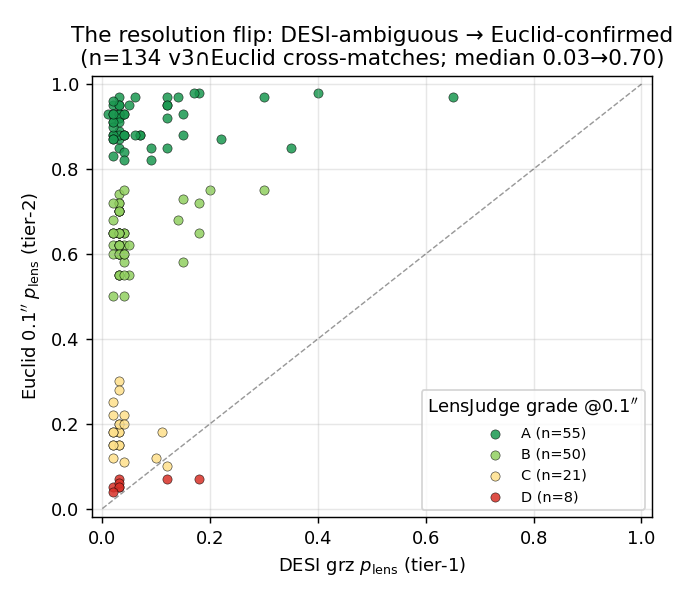
\includegraphics[width=0.485\linewidth]{figures/euclid_flip.png}\hfill
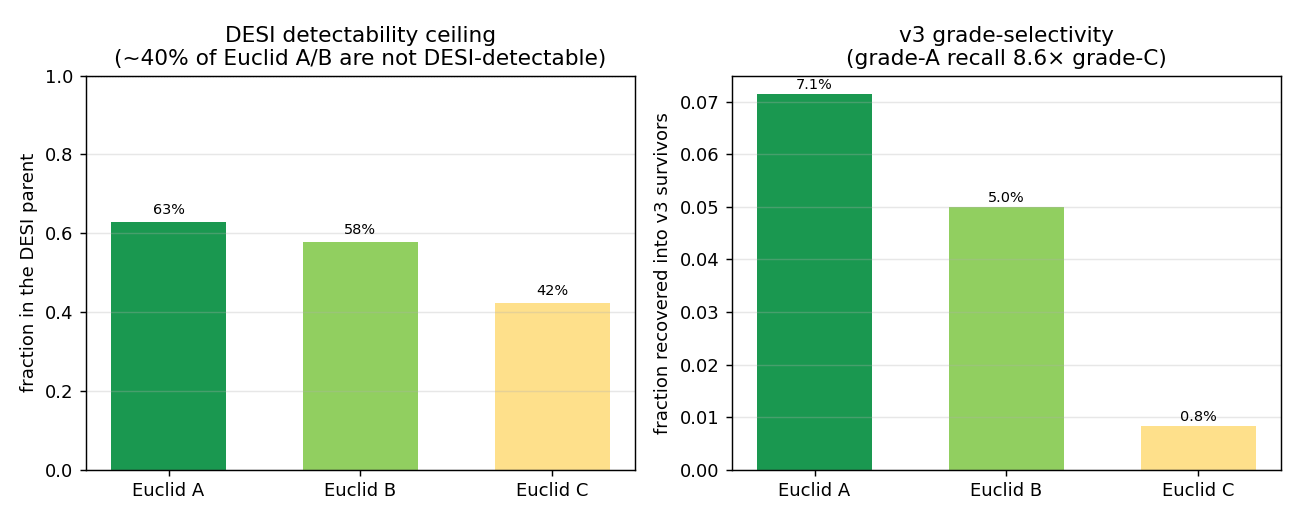
\includegraphics[width=0.485\linewidth]{figures/euclid_recall.png}
\caption{\textbf{The resolution lever.} Left: the DESI$\to$Euclid $p_{\rm lens}$ flip on the real
v3$\cap$Euclid cross-matches --- nearly every object is DESI-ambiguous ($x\!\lesssim\!0.2$) but
Euclid-confirmed ($y\!\gtrsim\!0.6$). Right: Euclid grade-resolved recall --- the DESI detectability
ceiling ($\sim$40\% of Euclid A/B missing from the parent) and v3's $8.6\times$ grade-A-over-C
survivor selectivity.}
\label{fig:euclid_flip}\label{fig:euclid_recall}
\end{figure}

\paragraph{Honest limits and a selection-bias correction (D6, D3).}
\label{sec:v3limits}
The v3-vs-v2 mimic-separation gains above are real, but the cross-model comparison demands one
correction (Table~\ref{tab:progression}). The seed mimic-FPR metric is \emph{selection-biased}: the
seed bank \emph{is} the set the v2/v3 ensemble scored high, so it saturates their threshold and
deflates their recovery, while a model less central to the selection (a single random-negative
EfficientNet) looks artificially strong there --- so any ``$N\times$ over the original published
models'' read off the seed is invalid and we do not claim it. The trustworthy comparison is the
\emph{independent} Euclid grade-A-vs-C AUC: the original CNN, v2-lean, v3blend8, and the head all
sit at $0.61$--$0.66$, within $\sim$1 standard error ($n_A{=}66$) --- statistically
indistinguishable at the hardest distinction. v3 \emph{does} clearly beat the original on the broad
mimic population (DR10-eval recovery $0.60\!\to\!0.89$), i.e.\ it yields a meaningfully cleaner
candidate list to vet, but it has no significant edge at the resolution-bounded discovery frontier.
Finally, v3 is \textbf{DECam-specific}: a DR11-\emph{north} (BASS/MzLS) sweep shows systematic
under-scoring and zero Euclid-A/B in its top-30 --- north-footprint deployment needs instrument-
native retraining.

\begin{figure}[t]\centering
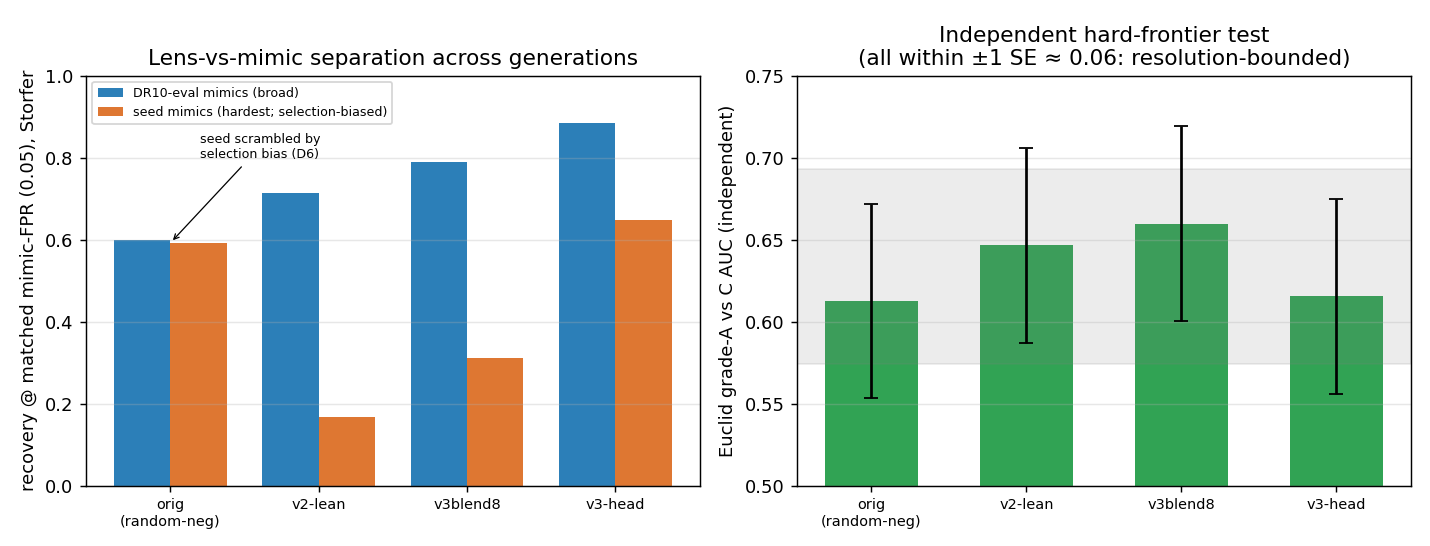
\includegraphics[width=0.95\linewidth]{figures/model_progression.png}
\caption{\textbf{Candidate quality across model generations.} Left: recovery@matched-mimic-FPR(0.05)
on the broad DR10-eval mimics (clear orig$\to$v2$\to$v3 progression) and on the curated seed mimics
(scrambled by the selection bias --- the seed is what the v2/v3 ensemble scored high). Right: the
\emph{independent} Euclid grade-A-vs-C AUC --- all four models lie within $\sim$1 standard error,
i.e.\ the hardest real-vs-mimic distinction is resolution-bounded for every model.}
\label{fig:progression}
\end{figure}

\begin{table}[t]\centering
\caption{Candidate quality across model generations (D6). recovery@matched-mimic-FPR(0.05) and the \emph{independent} Euclid grade-A-vs-C AUC. The seed column is selection-biased (the seed bank is what the v2/v3 ensemble scored high), so orig-vs-v3 there is invalid; the trustworthy comparison is the Euclid AUC, where all models sit within $\sim$1\,SE ($\approx$0.06, $n_A{=}66$).}
\label{tab:progression}\small
\begin{tabular}{lcccc}
\toprule
model & seed mimic@0.05 & DR10-eval@0.05 & DR10-eval@0.05 & Euclid A-vs-C\\
 & (Storfer) & (Storfer) & (Inchausti) & AUC (indep.)\\
\midrule
orig (random-neg CNN) & 0.592 & 0.598 & 0.640 & 0.613\\
v2-lean & 0.168 & 0.713 & 0.856 & 0.647\\
v3blend8 & 0.312 & 0.790 & 0.896 & 0.660\\
v3-head & 0.647 & 0.885 & 0.922 & 0.615\\
\bottomrule
\end{tabular}
\end{table}


\paragraph{Vetting: LensJudge v2 (summary).}
\label{sec:v3vetting}
The Euclid cross-validation above rests on the v2 upgrade of the \texttt{lensjudge} agentic vetter,
summarised here (full detail in \texttt{lensjudge/V2\_FINDINGS.md}). Three changes carry it:
(i) a \emph{two-tier high-res escalation} (DESI grz tier-1, Euclid $0.1''$ tier-2 when coverage
exists), live-validated as the $p_{\rm lens}$ flip; (ii) a rubric tuned to the dominant failure
modes (LRG+companion/ring/spiral/blend), which lifts lens-vs-mimic discrimination by $+0.196$ AUC
over the v1 grader on a frozen labelled benchmark; and (iii) an agency ablation showing the agentic
loop is unnecessary for \emph{detection} (a one-shot direct grader matches it $6\times$ cheaper) but
essential for \emph{mimic adjudication} --- motivating the deployed cascade (cheap direct triage
$+$ agentic v2 on survivors $+$ Euclid escalation by coverage).
